\section{Dynamical Quantum Phase Transitions}
Dynamical quantum phase transitions (DQPT) are non-equilibrium phase transitions in quantum many-body systems that occour on transient time scales and are driven by progressing time as opposed to conventional phase transitions, which are driven by parameters such as temperature or pressure. 

At the phase transition certain physical quantities become non-analytic as a function of time. We begin by taking a closer look at the relevant physical quantities.

For more conventional equilibrium phase transitions the central object is the partition function
\begin{equation}
    \label{eq:partition}
    Z = \yx{Tr}\left(\exp\left(-\beta\hat{H}(\alpha)\right)\right)= \exp\left(-\beta Nf(\beta,\alpha)\right)
\end{equation}
with the inverse of the temperature $\beta=\frac{1}{T}$, a Hamiltonian $\hat{H}$ that depends on a set of parameters $\alpha$, the system size $N$ and the free energy density $f(\alpha,\beta)$. If $f(\alpha,\beta)$ becomes non-analytic as a function of the parameters $\alpha$ and at zero-temperature, one speaks of a quantum phase transition. For dynamical phase transitions we define quantities that are formally similiar to the partition function. Consider a many-body system with Hamiltonian $H_0$ in its ground state $\Psi_0$. In a process called quantum quench the Hamiltonian is changed nearly instantaneously to $H$ at $t = 0$. Following the quench the state will evolve according to the Schroedinger equation with $\ket{\Psi_0(t)} = e^{-i\hat{H}t}\ket{\Psi_0}$. The amplitude and probability to return to the ground state at time $t$ are then termed Loschmidt amplitude and Loschmidt echo
\begin{align}
    \mathcal{G}(t) &= \bra{\Psi_0}e^{-i\hat{H}t}\ket{\Psi_0}, \\
    \mathcal{L}(t) &= \left|\bra{\Psi_0}\ket{\Psi_0(t)}\right|^2 .
\end{align}
The Loschmidt echo has an exponential dependence on system size $N$, revealing the formal similarity to the partition function \eqref{eq:partition} after defining the Loschmidt rate $\lambda(t)$ through
\begin{equation}
    \mathcal{L} = e^{-N\lambda(t)}.
\end{equation}
The DQPTs will show up as non-analytical points in the Loschmidt rate, in analogy with critical points in the equilibrium phase transitions.
\subsubsection{Exercise 1}
The rate function $g(t)$ in $\mathcal{G}(t) = e^{-Ng(t)}$ is connected to the Loschmidt rate with $\lambda(t) = 2\Re{[g(t)]}$, following directly from the definitions
\begin{equation}
    \mathcal{L}(t) = \abs{\mathcal{G}(t)}^2 = e^{-Ng(t)}e^{-Ng^*(t)} = e^{-2N\Re{[g(t)]}} = e^{-N\lambda(t)}.
\end{equation}
For systems with $N_\mathrm{gs}$ degenerate ground states $\Psi_i$ the Loschmidt echo is the probability to return to any of the ground states and therefore sums over all return probalities
\begin{equation}
    \mathcal{L}(t) = \sum^{N_\mathrm{gs}-1}_{i=0}\left|\bra{\Psi_i}\ket{\Psi_0(t)}\right|^2.
\end{equation}
The total Loschmidt rate $\lambda(t)$ is still extracted by taking the logarithm $\lambda(t) = - \frac{1}{N}\ln\mathcal{L}(t)$, however, the additional ground states allow us to introduce individual rates $\lambda_i(t)$
\begin{equation}
    e^{-N\lambda_i(t)} = \left|\bra{\Psi_i}\ket{\Psi_0(t)}\right|^2.
\end{equation}
\subsubsection{Exercise 2}
In the thermodynamic limit $N \to \infty$ the total Loschmidt rate $\lambda(t)$ becomes the smallest individual rate $\lambda(t) = \operatorname{min}[\lambda_i(t)]$. This equality is shown by factoring out the term $e^{-N\lambda_\mathrm{min}}$ in the Loschmidt definition, ensuring that all remaining exponential terms have a negative argument $-N(\lambda_i - \lambda_\mathrm{min}) < 0$. Then the product formula $\ln a\cdot b = \ln a + \ln b$ is applied.
\begin{equation*}
    \lambda(t) = - \lim_{N\to\infty}\frac{1}{N}\ln \sum^{N_\mathrm{gs}-1}_{i=0}e^{-N\lambda_i} = - \lim_{N\to\infty}\frac{1}{N}\ln \left[e^{-N\lambda_\mathrm{min}}\sum^{N_\mathrm{gs}-1}_{i=0}e^{-N(\lambda_i-\lambda_\mathrm{min})}\right]
\end{equation*}
 All of the terms, except the minimum rate, vanish in the limit after using $\ln 1 + x \simeq x$ for $x \ll 1$.
 \begin{equation*}
    \lambda(t) = \lambda_\mathrm{min} - \lim_{N\to\infty}\frac{1}{N}\ln\left[1 + \sum^{N_\mathrm{gs}-1}_{i=\neq\mathrm{min}}e^{-N(\lambda_i-\lambda_\mathrm{min})}\right] \simeq \lambda_\mathrm{min} + \lim_{N\to\infty} \sum^{N_\mathrm{gs}-1}_{i=\neq\mathrm{min}} e^{-N(\lambda_i - \lambda_\mathrm{min})} = \lambda_\mathrm{min}
 \end{equation*}
\section{Transverse Field Ising Model}
The transverse field Ising model (TFI) describes a linear chain of $N$ qubits with nearest neighbor interaction. Due to its known analytical solution it is a suitable system to test the performance of numerical simulations, including our state vector simulation with trotterization. The TFI Hamiltonian $\hat{H}$ reads
\begin{equation}
    \label{eq:tfi}
    \hat{H} = -\frac{1}{2}\sum_{\left<i,j\right>}Z_iZ_j - \frac{g}{2}\sum_iX_i
\end{equation}
with $g$ being the strength of the transverse field. The $Z_iZ_j$ interaction strength is constant at unity. The system is symmetric under the parity operator 
\begin{equation}
    \hat{P} = \bigotimes_i X_i
\end{equation}
with spectrum $\{-1, 1\}$, since the commutator $[\hat{H}, \hat{P}] = 0$ vanishes. This is derived using the identities $X^2_i = \mathbb{1}$, $\hat{P} = \hat{P}^\dagger$ and $X_iZ_iX_i = -Z_i$. Each interaction term consists of two $Z_i$ matrices. This cancels out the negative sign when using the latter identity in computing $\hat{P}\hat{H}$.
\subsubsection{Exercise 3}
\begin{equation}
    \left[\hat{H}\hat{P} - \hat{P}\hat{H}\right]\hat{P}^\dagger = \hat{H} - \hat{P}\hat{H}\hat{P}^\dagger = \hat{H} - \hat{H} = 0 \Rightarrow [\hat{H}, \hat{P}] = 0
\end{equation}
In the limit $g = 0$ the ground states of $\hat{H}$ are $\ket{\Psi_0} = \ket{0\ldots 0}$ and $\ket{\Psi_1} = \ket{1\ldots1}$, while for $g \to \infty$ only one ground state $\ket{\Psi_+} = \ket{+\ldots+}$ exists. The magnetization of the system is the average spin orientation
\begin{equation}
    m_z = \frac{1}{N}\sum_i Z_i.
\end{equation}
For the ground states above it takes the values $m^0_z = \bra{\Psi_0}\frac{1}{N}\sum_i Z_i\ket{\Psi_0} = -1$, $m^1_z = +1$ and $m^+_z = 0$. $\ket{\Psi_+}$ has parity symmetry but no magnetization, while the states $\Psi_0$ and $\Psi_1$ have no parity symmetry but finite magnetization. This indicates a symmetry-broken ferromagnetic phase with $m_z \neq 0$ for some critical field strength $g_c$. To find the critical point the Hamiltonian is reexpressed with a new set of Ising variables
\begin{equation}
    \label{eq:ising}
    \tilde{Z_n} = \bigotimes_{i \leq n} X_i \quad \tilde{X_n} = Z_nZ_{n+1}
\end{equation}
to expose its self-dual structure. For identical behavior these variables need to share the same anticommutation relation $\{Z_i, X_i\} = 0$ as the original variables. Note that $\{Z_i, X_j\} = 0$ for any $i$ and $j$, as the operators act on different qubits. 
\subsubsection{Exercise 4}
The new anticommutator $\{\tilde{Z}_i, \tilde{X}_i\}$ is evaluated by factoring out the old anticommutator
\begin{equation}
    \left\{\tilde{Z_n}, \tilde{X_n}\right\} = \bigotimes_{i \leq n}X_iZ_nZ_{n+1} + Z_nZ_{n+1}\bigotimes_{i \leq n}X_i = \left[X_nZ_n + Z_nX_n\right]Z_{n+1}\bigotimes_{i \leq n-1}X_i = 0.
\end{equation}
The Hamiltonian $H$ now has the two forms where the second form can be rescaled to $\hat{\tilde{H}}$ through division with with $g$.
\begin{align}
    \hat{H} &= -\frac{1}{2}\sum^{N}_{i=1}Z_iZ_{i+1} - \frac{g}{2}\sum^N_{i=1}X_i\\
    &= - \frac{1}{2}\sum^{N}_{n=1}\tilde{X}_n - \frac{g}{2}\sum^{N}_{n=1}\tilde{Z}_n\tilde{Z}_{n+1} \\
    \hat{\tilde{H}} &= - \frac{1}{2}\sum^{N}_{n=1}\tilde{Z}_n\tilde{Z}_{n+1} - \frac{1}{2g}\sum^{N}_{n=1}\tilde{X}_n 
\end{align}
Multiplying a Hamiltonian does not change the dynamics of the system. The absolute energy scale is an arbitrary choice, therefore only the relative magnitude between the Hamiltonian terms is physical. Specifically, at the critical field value $g_c$ both Hamiltonians $\hat{H}$ and $\hat{\tilde{H}}$ predict the same phase transition. By comparison the critical field has to assume $g_c = \frac{1}{g_c} = 1$.
\subsubsection{Exercise 5}
The predictions for paramagnetic and ferromagnetic states in the TFI model have been made without considering any environment. For a canonical system at finite temperatures, the ferromagnetic order is not expected to survive over long ranges. In the 1D model the energy associated with a single domain wall is set by the $Z_iZ_{i+1}$ interaction term.
\begin{equation}
    \Delta E = - \frac{1}{2}\left<Z_iZ_{i+1}\right> = \frac{1}{2}
\end{equation}
In addition to the energy cost, every domain wall will add to the entropy $S$ of the chain. While the energy $E$ does not increase with system size $N$, the number of domain walls and the entropy does. For a system in contact with a thermal bath, the free energy $F = E - TS$ is minimized. The presence of many domain walls is therefore prefered due the higher entropy, despite the associated energy cost. This prevents ferromagnetic phases to extend over long distances.
\section{DQPTs in the TFI using Cirq}
In this section we study the time evolution generated by the Hamiltonian from equation \eqref{eq:tfi}.
\subsection{Implementing the time evolution}
As in day 1 of the FOPRA, we will perform a Trotter decomposition of the time evolution operator $\hat{U}(t)$. We may write 
\begin{equation}
U(t) = e^{-\iu\hat{H}t} = \left(e^{-\iu\hat{H}dt}\right)^{\frac{t}{dt}} = \left(e^{\hat{A}+\hat{B}}\right)^\frac{t}{dt}
\end{equation}
where $\hat{A} = -\frac{g}{2}dt \sum_i X_i$ and $\hat{B} = -\frac{1}{2}dt \sum_{\expval{i,j}}Z_iZ_j$.
\subsubsection{Exercises 6 and 7}
To implement this unitary in Cirq we first create a circuit that represents the evolution of the system by a small time step $dt$ up to second order Trotterization. To benchmark our results, we simulate the time evolution and extract the magnetization $m_z(t)$ as a function of time for a system of $L=10$ at $g=2$, starting from an initial state $\ket{\psi_0} = \ket{0...0}$ of all spins down. As seen in figure \ref{fig:ex6d2} the trotterization with timestep $dt = 0.25$ agrees very well with the exact solution obtained through diagonalizing the Hamiltonian.
\begin{figure}[h]
    \centering
    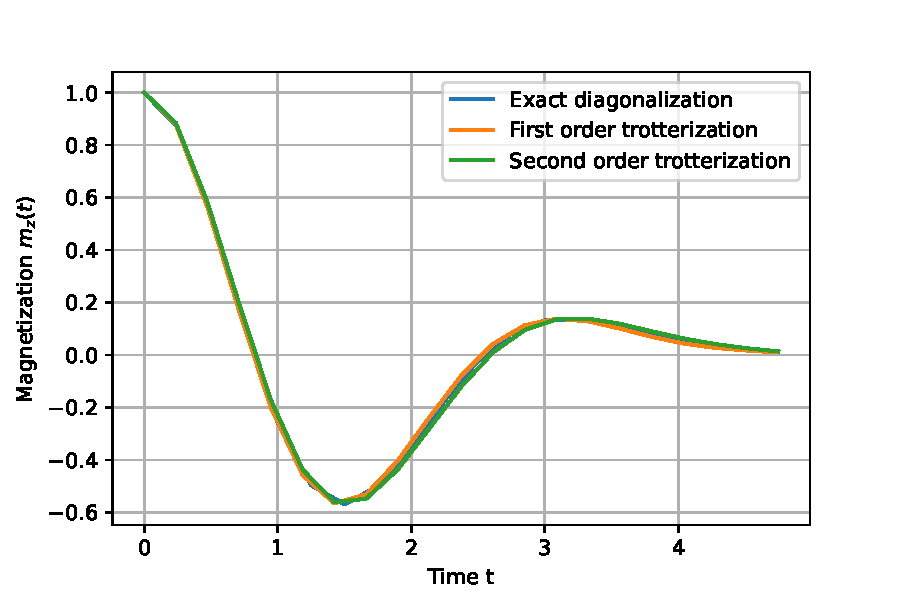
\includegraphics[width=0.6\textwidth]{tex/figures/Ex6d2.pdf}
    \caption{Magnetization $m_z$ over time $t$ for a $L = 10$ qubit chain in the tranverse field Ising model. First and second order trotterization delivers very accurate results compared to the exact evolution computed with diagonalization.}
    \label{fig:ex6d2}
\end{figure}

\subsubsection{Exercise 8}
We now want to evaluate the Loschmidt rate for an initial Hamiltonian $\hat{H}|_{g_0}$, where the two degenerate
ferromagnetic ground states are $\ket{\psi_0} =\ket{0...0}$ and $\ket{\psi_0} =\ket{1...1}$. Using the same time evolution as above, we extract the simulated Loschmidt rate by projecting back onto the ground state manifold. To study the results, we first plot the simulated Loschmidt rates for different system sizes while keeping the transverse field strength constant. We plot the results in figure \ref{fig:Loschmidt}. We can clearly see DQPTs occuring at $ts\approx1.8$ regardless of the system size.
\begin{figure}[h]
    \centering
    \caption{Simulated Loschmidt rates for different system sizes L with a strength of the transverse field g=2.}
    \label{fig:Loschmidt}
    \addtocounter{figure}{-1}
    \begin{subfigure}[t]{0.48\textwidth}
        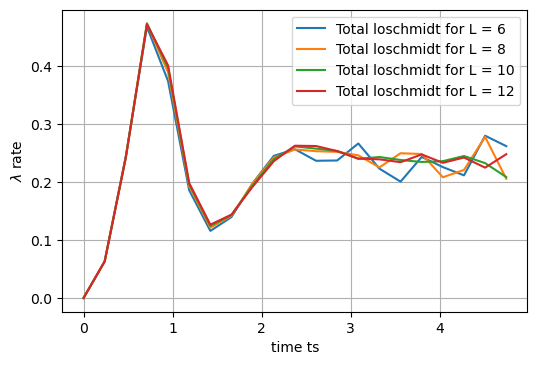
\includegraphics[width=\textwidth]{tex/figures/Lochschmidt.png}
        \caption{Loschmidt rate $\lambda(t)$}
    \end{subfigure}\\
    \begin{subfigure}[t]{0.48\textwidth}
        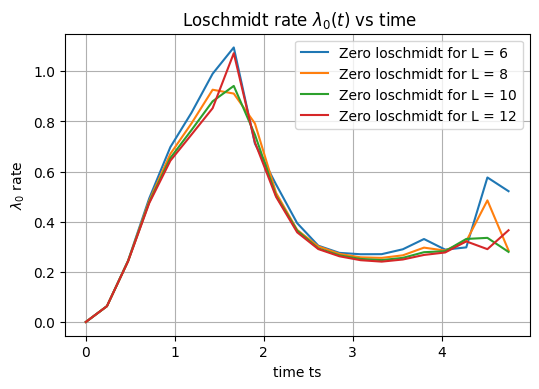
\includegraphics[width=\textwidth]{tex/figures/Loschmidt0.png}
         \caption{Loschmidt rate $\lambda_0(t)$}
    \end{subfigure}
    \begin{subfigure}[t]{0.48\textwidth}
        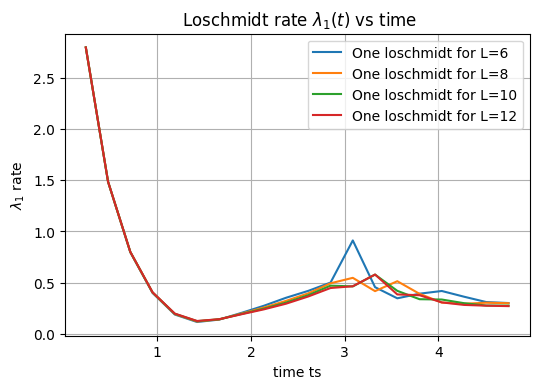
\includegraphics[width=\textwidth]{tex/figures/Loschmidt1.png}
         \caption{Loschmidt rate $\lambda_1(t)$}
    \end{subfigure}
\end{figure}

Next, in figure \ref{fig:LoschmidtManyGs} we do the same but keep the system size fixed and varying the transverse field strength. Again we can clearly see DQPTs occuring for $g>1$.

\begin{figure}[h]
    \centering
    \caption{Simulated Loschmidt rates for fixed sytsem size of L=12 and varying strength of the transverse field g=2.}
    \label{fig:LoschmidtManyGs}
    \addtocounter{figure}{-1}
    \begin{subfigure}[t]{0.48\textwidth}
        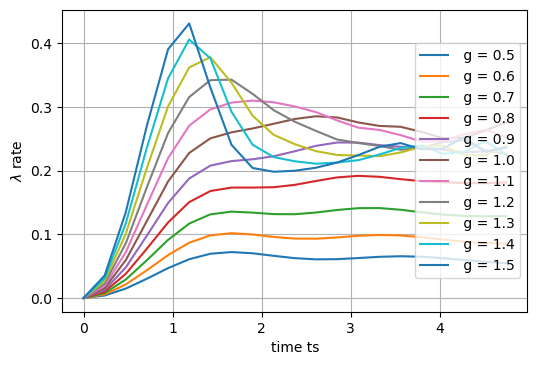
\includegraphics[width=\textwidth]{tex/figures/LochschmidtManyGs.png}
        \caption{Loschmidt rate $\lambda(t)$}
    \end{subfigure}\\
    \begin{subfigure}[t]{0.48\textwidth}
        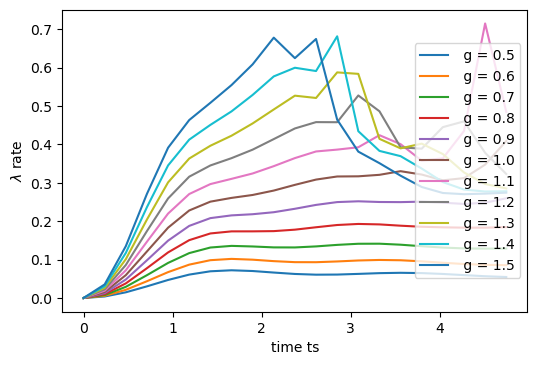
\includegraphics[width=\textwidth]{tex/figures/Lochschmidt0ManyGs.png}
         \caption{Loschmidt rate $\lambda_0(t)$}
    \end{subfigure}
    \begin{subfigure}[t]{0.48\textwidth}
        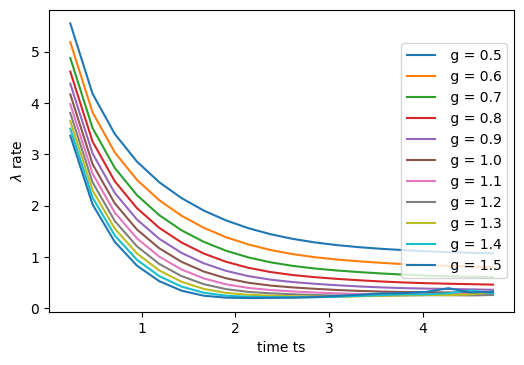
\includegraphics[width=\textwidth]{tex/figures/Lochschmidt1ManyGs.png}
         \caption{Loschmidt rate $\lambda_1(t)$}
    \end{subfigure}
\end{figure}

\subsubsection{Exercise 9}
Now we determine both the magnetization and Loschmidt echo as a function of time again, this time via repeated measurements. Figure \ref{fig:LoschMagComp} shows the results, which are essentially identical to the results from the exact solution. 
\begin{figure}[h!]
    \centering
    \caption{Loschmidt echo and magnetization as a function of time reconstructed using simulation of the exact solutions and using repeated measurements respectively.}
    \label{fig:LoschMagComp}
    \addtocounter{figure}{-1}
    \begin{subfigure}[t]{0.48\textwidth}
        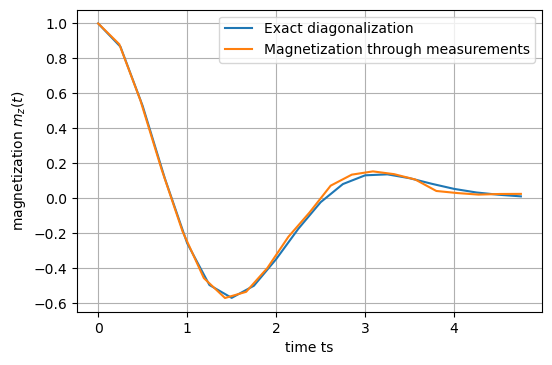
\includegraphics[width=\textwidth]{tex/figures/Magnetization2.png}
        \caption{Magnetization as a function of time.}
    \end{subfigure}
    \begin{subfigure}[t]{0.48\textwidth}
        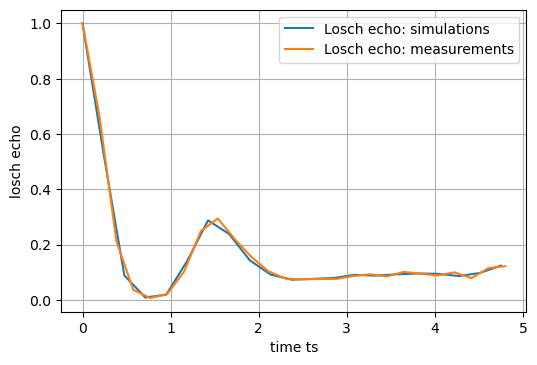
\includegraphics[width=\textwidth]{tex/figures/LoschEchoVSTime.png}
         \caption{Loschmidt echo as a function of time.}
    \end{subfigure}
\end{figure}

To determine how much sampling is in principle necessary to obtain accurate results, we notice that the maximum value of the total Loschmidt rate is approximately 0.5. Therefore,
\begin{equation}
    \frac{\min(\#\yx{of} \ket{0...0} \yx{or}\ket{1...1}}{\#\yx{of~samplings}} \approx \exp\left(-0.5N\right)
\end{equation}
In order to get accurate results, the expected frequency of getting the state $\ket{0...0}$ or $\ket{1..1}$must not be too small. In practice, we could set the expected frequency of ground state to be larger than 10, then the sampling times should fulfill.
\begin{equation}
    \#\yx{of~samplings} \geq 10\exp\left(-0.5N\right)
\end{equation}

\subsubsection{Exercise 10}
By putting both the magnetization and Loschmidt echo in the same plot, as seen in figure \ref{fig:MagAndLosch} we find that the turning point of magnetization (at around t = 1.5) corresponds to the second turning point of $\lambda(t)$.
\begin{figure}[h]
    \centering
    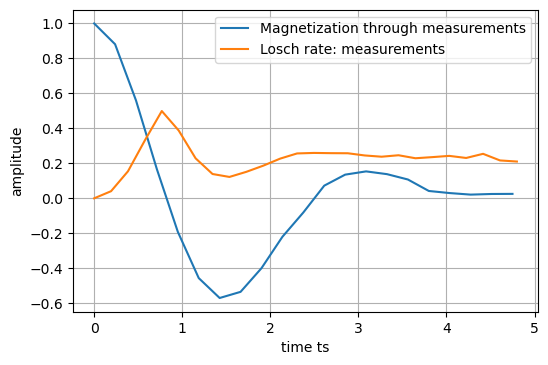
\includegraphics[width= 0.6\textwidth]{tex/figures/MagAndLosch.png}
    \caption{Magnetization and Loschmidt echo as a function of time.}
    \label{fig:MagAndLosch}
\end{figure}

\section{Tracking Entanglement Production}

After the quantum quench takes place, our state evolves from the initial product state to a system with higher entanglement. Due to this effect, it becomes increasingly harder to express the system using classical methods such as matrix product states (MPS).

In this exercise we will quantify the half-chain entanglement using the second Renyi entropy. The reduced density matrix of the subsystem $l$ in consideration is defined as:

\begin{equation}
    \rho_l = \Tr_r{[\rho]}
    \label{eq:reduced_matrix}
\end{equation}

Where the trace $\operatorname{Tr}_r$ is taken over the qubits that are not part of our subsystem, and $\rho$ is the matrix of the full system. Then, the second Renyi entropy is defined as \cite{manual}:

\begin{equation}
    S^{(2)} = - \log(\Tr{[\rho_l^2]})
    \label{eq:renyi_entropy}
\end{equation}


\subsubsection{Exercise 17}

From \cite{renyi_paper} we see there is an alternative way of obtaining the Renyi entropy through randomized measurements. First, we define the 1-qubit unitary gates from the circular unitary ensemble (CUE) acting on qubit $i$ defined as:

\begin{equation}
    \begin{split}
    U_i(a,b,c) & = \begin{pmatrix} e^{ia} \cos(b)  & e^{ic} \sin(b) \\ -e^{-ic} \sin(b) & e^{-ia} \cos(b) \end{pmatrix}. \\
     & = e^{i(a+c)Z/2} e^{ibY} e^{i(a-c)Z/2}
    \end{split}
\end{equation}

Where $a$ and $c$ are uniformly distributed over [$0$, $2\pi$], and $b$ is uniformly distributed over [0, $\pi/2$]\\

The second equality is useful for its code implementation. \textbf{Note: } This matrix differs by a minus sign from the one provided in the lab manual, since the gates proposed for cirq do not coincide.\\

The three parameters are sampled randomly generating a different $U_i$ to be applied on each of the qubits of the system. Then the subsystem is measured in the computational basis. From this, the probabilities $P_U(s_A)$ of measuring the bitstrings $s_A$ on the subsystem are obtained. With this information, an estimation of the purity ($\Tr{[\rho_l^2]}$) of the measured subsystem is obtained as:

\begin{equation}
    \label{eq:estimation_purity}
    X = 2^{L_a} \sum_{s_A, s^{'}_A} (-2)^{-D(s_A, s^{'}_A)} P_U(s_A) P_U(s^{'}_A)
\end{equation}

Where $D(s_A, s^{'}_A)$ represents the hamming distance between the bistrings $s_A$ and $s^{'}_A$, i.e. the number of different bits between the two bitstrings. \textbf{Important}: the sum runs over all possible tuples containing the combinations of bitstrings, this includes the cases where $s_A = s^{'}_A$ and symmetric cases such as $(s_A, s^{'}_A)$ and $(s^{'}_A, s_A)$. \\

This procedure is repeated for several independent realizations of the CUE unitaries, and the purity average $\overline{X}$ is used to obtain the final expression for the second Renyi entropy as:

\begin{equation}
    \label{eq:renyi_entropy_estimation}
    S^{(2)} = - \log(\overline{X})
\end{equation}

For its implementation in cirq, we write a function \texttt{U2\_CUE(qubit, symbs)} that applies the unitary $U_i$ from CUE to the qubit in the parameter \texttt{qubit}. The unitary is generated from the list of three parameters provided through \texttt{symbs}. Then, the hamming function defined above is also implemented in the code as \texttt{hamming(s1,s2)} where \texttt{s1} and \texttt{s2} are the two bitstrings to compare.\\

The time evolution of our system is studied under the trotterization from previous exercises using the simple evolution method and the Renyi entropy is calculated after each time step. For this simulation, we choose a total of 2000 measurement
repetitions, and 200 different instances of the CUE chosen using random generators over the correspondent ranges of the parameters.\\

The following graph shows the simulation for a hamiltonian using $g = 2$ applied on a two-qubit system that evolves  with a time step of $\delta t = 0.25$ for $N = \operatorname{int}(5/\delta t)$ time steps. For comparison, the exact value of the Renyi entropy was calculated through the density matrix of the total system after each time step provided by the function \texttt{cirq.Simulator().simulate}.

\begin{figure}[h]
    \label{fig:renyi_entropy}
    \centering
    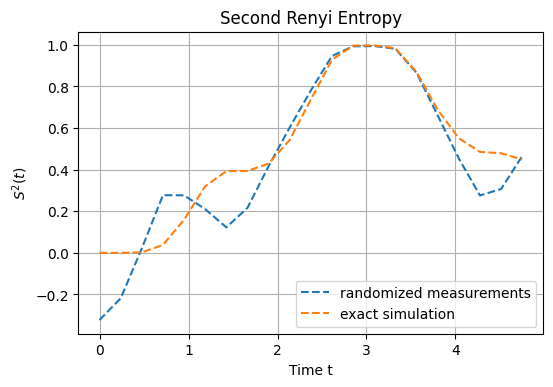
\includegraphics[width=0.8\textwidth]{tex/figures/exercise17.png}
    \caption{Second Renyi entropy simulation for a two-qubit system evolved by a first degree troterization}
\end{figure}